\documentclass{standalone}
\usepackage{tikz}
\usetikzlibrary{patterns, positioning}


\begin{document}
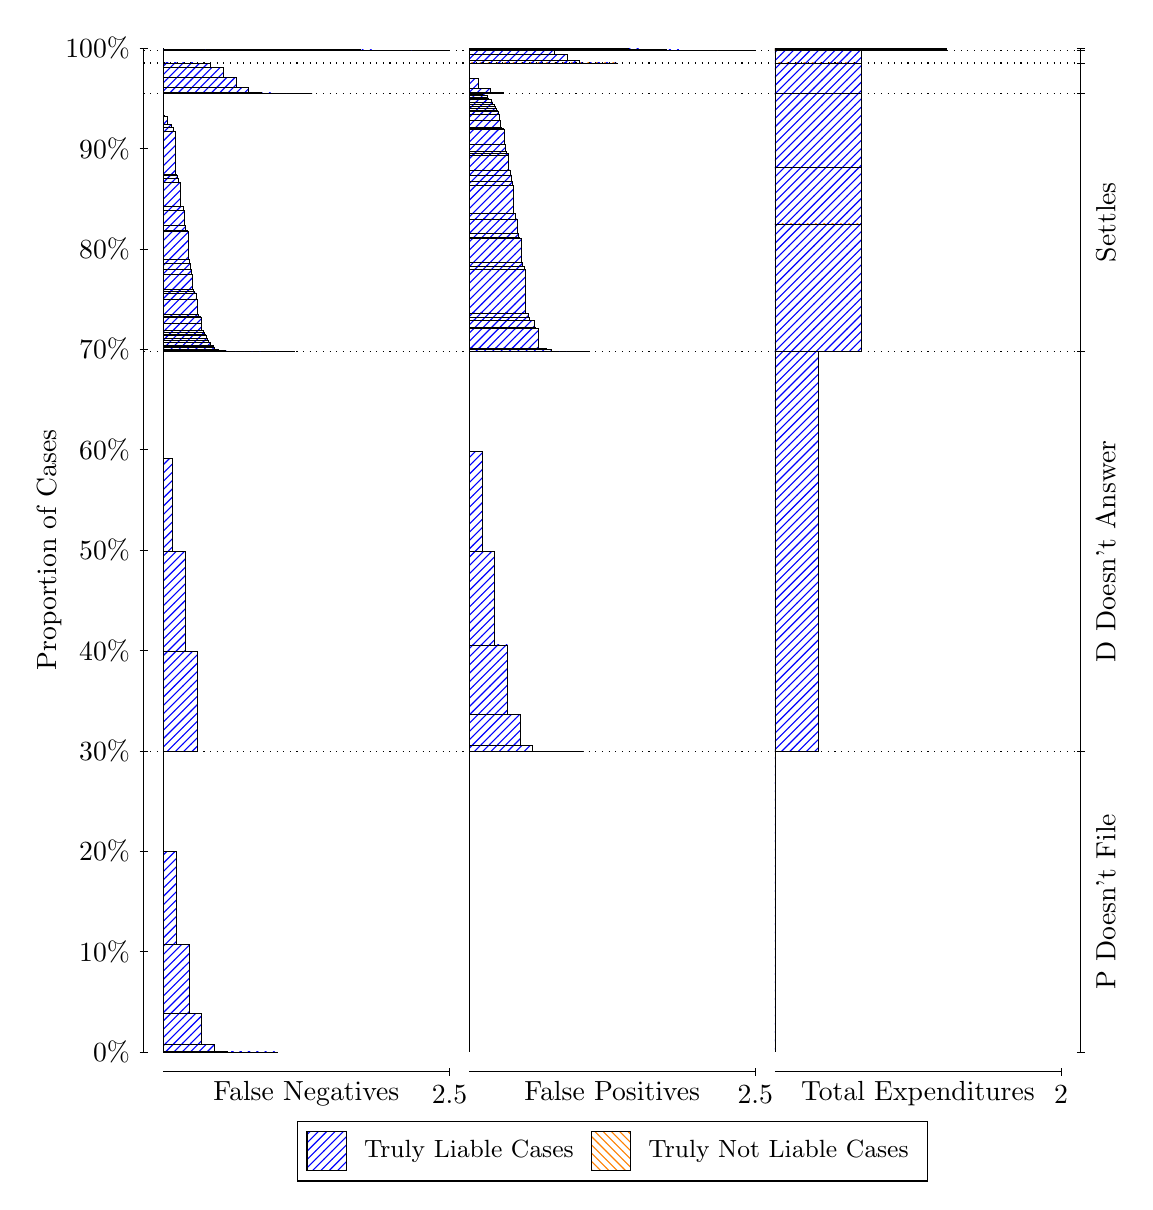
\begin{tikzpicture}
\draw[black, very thin] (1.5,1.75) -- (1.5,14.5);
\node[rotate=90, text=black, anchor=center] at (0.3, 8.125) {Proportion of Cases};
\draw[black, very thin] (1.45,1.75) -- (1.55,1.75);
\node[text=black, anchor=east] at (1.45, 1.75) {0\%};
\draw[black, very thin] (1.45,3.025) -- (1.55,3.025);
\node[text=black, anchor=east] at (1.45, 3.025) {10\%};
\draw[black, very thin] (1.45,4.3) -- (1.55,4.3);
\node[text=black, anchor=east] at (1.45, 4.3) {20\%};
\draw[black, very thin] (1.45,5.575) -- (1.55,5.575);
\node[text=black, anchor=east] at (1.45, 5.575) {30\%};
\draw[black, very thin] (1.45,6.85) -- (1.55,6.85);
\node[text=black, anchor=east] at (1.45, 6.85) {40\%};
\draw[black, very thin] (1.45,8.125) -- (1.55,8.125);
\node[text=black, anchor=east] at (1.45, 8.125) {50\%};
\draw[black, very thin] (1.45,9.4) -- (1.55,9.4);
\node[text=black, anchor=east] at (1.45, 9.4) {60\%};
\draw[black, very thin] (1.45,10.675) -- (1.55,10.675);
\node[text=black, anchor=east] at (1.45, 10.675) {70\%};
\draw[black, very thin] (1.45,11.95) -- (1.55,11.95);
\node[text=black, anchor=east] at (1.45, 11.95) {80\%};
\draw[black, very thin] (1.45,13.225) -- (1.55,13.225);
\node[text=black, anchor=east] at (1.45, 13.225) {90\%};
\draw[black, very thin] (1.45,14.5) -- (1.55,14.5);
\node[text=black, anchor=east] at (1.45, 14.5) {100\%};

\draw[black, very thin] (13.4,1.75) -- (13.4,14.5);
\draw[black, very thin] (13.35,1.75) -- (13.45,1.75);
\node[anchor=west] at (13.35, 1.75) {};
\draw[black, very thin] (13.35,5.563) -- (13.45,5.563);
\node[anchor=west] at (13.35, 5.563) {};
\draw[black, very thin] (13.35,10.651) -- (13.45,10.651);
\node[anchor=west] at (13.35, 10.651) {};
\draw[black, very thin] (13.35,13.928) -- (13.45,13.928);
\node[anchor=west] at (13.35, 13.928) {};
\draw[black, very thin] (13.35,14.31) -- (13.45,14.31);
\node[anchor=west] at (13.35, 14.31) {};
\draw[black, very thin] (13.35,14.474) -- (13.45,14.474);
\node[anchor=west] at (13.35, 14.474) {};
\draw[black, very thin] (13.35,14.5) -- (13.45,14.5);
\node[anchor=west] at (13.35, 14.5) {};

\draw[black, very thin, pattern color=blue, pattern=north east lines] (1.75,1.75) rectangle (3.2033,1.75);
\draw[black, very thin, pattern color=blue, pattern=north east lines] (1.75,1.75) rectangle (3.0419,1.75);
\draw[black, very thin, pattern color=blue, pattern=north east lines] (1.75,1.75) rectangle (2.8804,1.75);
\draw[black, very thin, pattern color=blue, pattern=north east lines] (1.75,1.75) rectangle (2.7189,1.7503);
\draw[black, very thin, pattern color=blue, pattern=north east lines] (1.75,1.7503) rectangle (2.5574,1.7582);
\draw[black, very thin, pattern color=blue, pattern=north east lines] (1.75,1.7582) rectangle (2.3959,1.8434);
\draw[black, very thin, pattern color=blue, pattern=north east lines] (1.75,1.8434) rectangle (2.2344,2.2366);
\draw[black, very thin, pattern color=blue, pattern=north east lines] (1.75,2.2366) rectangle (2.073,3.1157);
\draw[black, very thin, pattern color=blue, pattern=north east lines] (1.75,3.1157) rectangle (1.9115,4.2995);
\draw[black, very thin, pattern color=orange, pattern=north west lines] (1.75,4.2995) rectangle (1.75,4.2995);
\draw[black, very thin, pattern color=blue, pattern=north east lines] (1.75,4.2995) rectangle (1.75,5.563);
\draw[black, very thin, pattern color=blue, pattern=north east lines] (1.75,5.563) rectangle (2.186,6.8376);
\draw[black, very thin, pattern color=blue, pattern=north east lines] (1.75,6.8376) rectangle (2.0245,8.1041);
\draw[black, very thin, pattern color=blue, pattern=north east lines] (1.75,8.1041) rectangle (1.863,9.2934);
\draw[black, very thin, pattern color=orange, pattern=north west lines] (1.75,9.2934) rectangle (1.75,9.2934);
\draw[black, very thin, pattern color=blue, pattern=north east lines] (1.75,9.2934) rectangle (1.75,10.651);
\draw[black, very thin, pattern color=blue, pattern=north east lines] (1.75,10.651) rectangle (3.4213,10.651);
\draw[black, very thin, pattern color=blue, pattern=north east lines] (1.75,10.651) rectangle (3.3487,10.651);
\draw[black, very thin, pattern color=blue, pattern=north east lines] (1.75,10.651) rectangle (3.276,10.651);
\draw[black, very thin, pattern color=blue, pattern=north east lines] (1.75,10.651) rectangle (3.2599,10.651);
\draw[black, very thin, pattern color=blue, pattern=north east lines] (1.75,10.651) rectangle (3.2033,10.651);
\draw[black, very thin, pattern color=blue, pattern=north east lines] (1.75,10.651) rectangle (3.1872,10.651);
\draw[black, very thin, pattern color=blue, pattern=north east lines] (1.75,10.651) rectangle (3.1307,10.651);
\draw[black, very thin, pattern color=blue, pattern=north east lines] (1.75,10.651) rectangle (3.1145,10.651);
\draw[black, very thin, pattern color=blue, pattern=north east lines] (1.75,10.651) rectangle (3.0984,10.651);
\draw[black, very thin, pattern color=blue, pattern=north east lines] (1.75,10.651) rectangle (3.058,10.651);
\draw[black, very thin, pattern color=blue, pattern=north east lines] (1.75,10.651) rectangle (3.0419,10.651);
\draw[black, very thin, pattern color=blue, pattern=north east lines] (1.75,10.651) rectangle (3.0257,10.651);
\draw[black, very thin, pattern color=blue, pattern=north east lines] (1.75,10.651) rectangle (2.9853,10.651);
\draw[black, very thin, pattern color=blue, pattern=north east lines] (1.75,10.651) rectangle (2.9692,10.651);
\draw[black, very thin, pattern color=blue, pattern=north east lines] (1.75,10.651) rectangle (2.953,10.651);
\draw[black, very thin, pattern color=blue, pattern=north east lines] (1.75,10.651) rectangle (2.9369,10.651);
\draw[black, very thin, pattern color=blue, pattern=north east lines] (1.75,10.651) rectangle (2.9127,10.651);
\draw[black, very thin, pattern color=blue, pattern=north east lines] (1.75,10.651) rectangle (2.8965,10.651);
\draw[black, very thin, pattern color=blue, pattern=north east lines] (1.75,10.651) rectangle (2.8804,10.651);
\draw[black, very thin, pattern color=blue, pattern=north east lines] (1.75,10.651) rectangle (2.8642,10.651);
\draw[black, very thin, pattern color=blue, pattern=north east lines] (1.75,10.651) rectangle (2.84,10.651);
\draw[black, very thin, pattern color=blue, pattern=north east lines] (1.75,10.651) rectangle (2.8239,10.651);
\draw[black, very thin, pattern color=blue, pattern=north east lines] (1.75,10.651) rectangle (2.8077,10.651);
\draw[black, very thin, pattern color=blue, pattern=north east lines] (1.75,10.651) rectangle (2.7916,10.651);
\draw[black, very thin, pattern color=blue, pattern=north east lines] (1.75,10.651) rectangle (2.7754,10.651);
\draw[black, very thin, pattern color=blue, pattern=north east lines] (1.75,10.651) rectangle (2.7673,10.651);
\draw[black, very thin, pattern color=blue, pattern=north east lines] (1.75,10.651) rectangle (2.7512,10.651);
\draw[black, very thin, pattern color=blue, pattern=north east lines] (1.75,10.651) rectangle (2.735,10.651);
\draw[black, very thin, pattern color=blue, pattern=north east lines] (1.75,10.651) rectangle (2.7189,10.651);
\draw[black, very thin, pattern color=blue, pattern=north east lines] (1.75,10.651) rectangle (2.7027,10.651);
\draw[black, very thin, pattern color=blue, pattern=north east lines] (1.75,10.651) rectangle (2.6785,10.651);
\draw[black, very thin, pattern color=blue, pattern=north east lines] (1.75,10.651) rectangle (2.6624,10.651);
\draw[black, very thin, pattern color=blue, pattern=north east lines] (1.75,10.651) rectangle (2.6462,10.651);
\draw[black, very thin, pattern color=blue, pattern=north east lines] (1.75,10.651) rectangle (2.6301,10.651);
\draw[black, very thin, pattern color=blue, pattern=north east lines] (1.75,10.651) rectangle (2.6139,10.652);
\draw[black, very thin, pattern color=blue, pattern=north east lines] (1.75,10.652) rectangle (2.6059,10.652);
\draw[black, very thin, pattern color=blue, pattern=north east lines] (1.75,10.652) rectangle (2.5897,10.652);
\draw[black, very thin, pattern color=blue, pattern=north east lines] (1.75,10.652) rectangle (2.5736,10.652);
\draw[black, very thin, pattern color=blue, pattern=north east lines] (1.75,10.652) rectangle (2.5574,10.653);
\draw[black, very thin, pattern color=blue, pattern=north east lines] (1.75,10.653) rectangle (2.5493,10.654);
\draw[black, very thin, pattern color=blue, pattern=north east lines] (1.75,10.654) rectangle (2.5413,10.656);
\draw[black, very thin, pattern color=blue, pattern=north east lines] (1.75,10.656) rectangle (2.517,10.656);
\draw[black, very thin, pattern color=blue, pattern=north east lines] (1.75,10.656) rectangle (2.5009,10.657);
\draw[black, very thin, pattern color=blue, pattern=north east lines] (1.75,10.657) rectangle (2.4847,10.659);
\draw[black, very thin, pattern color=blue, pattern=north east lines] (1.75,10.659) rectangle (2.4686,10.663);
\draw[black, very thin, pattern color=blue, pattern=north east lines] (1.75,10.663) rectangle (2.4524,10.673);
\draw[black, very thin, pattern color=blue, pattern=north east lines] (1.75,10.673) rectangle (2.4444,10.674);
\draw[black, very thin, pattern color=blue, pattern=north east lines] (1.75,10.674) rectangle (2.4282,10.675);
\draw[black, very thin, pattern color=blue, pattern=north east lines] (1.75,10.675) rectangle (2.4121,10.676);
\draw[black, very thin, pattern color=blue, pattern=north east lines] (1.75,10.676) rectangle (2.3959,10.704);
\draw[black, very thin, pattern color=blue, pattern=north east lines] (1.75,10.704) rectangle (2.3879,10.713);
\draw[black, very thin, pattern color=blue, pattern=north east lines] (1.75,10.713) rectangle (2.3798,10.727);
\draw[black, very thin, pattern color=blue, pattern=north east lines] (1.75,10.727) rectangle (2.3556,10.728);
\draw[black, very thin, pattern color=blue, pattern=north east lines] (1.75,10.728) rectangle (2.3394,10.763);
\draw[black, very thin, pattern color=blue, pattern=north east lines] (1.75,10.763) rectangle (2.3233,10.79);
\draw[black, very thin, pattern color=blue, pattern=north east lines] (1.75,10.79) rectangle (2.3071,10.817);
\draw[black, very thin, pattern color=blue, pattern=north east lines] (1.75,10.817) rectangle (2.291,10.848);
\draw[black, very thin, pattern color=blue, pattern=north east lines] (1.75,10.848) rectangle (2.2829,10.871);
\draw[black, very thin, pattern color=blue, pattern=north east lines] (1.75,10.871) rectangle (2.2667,10.886);
\draw[black, very thin, pattern color=blue, pattern=north east lines] (1.75,10.886) rectangle (2.2506,10.915);
\draw[black, very thin, pattern color=blue, pattern=north east lines] (1.75,10.915) rectangle (2.2344,11);
\draw[black, very thin, pattern color=blue, pattern=north east lines] (1.75,11) rectangle (2.2264,11.085);
\draw[black, very thin, pattern color=blue, pattern=north east lines] (1.75,11.085) rectangle (2.2183,11.099);
\draw[black, very thin, pattern color=blue, pattern=north east lines] (1.75,11.099) rectangle (2.1941,11.116);
\draw[black, very thin, pattern color=blue, pattern=north east lines] (1.75,11.116) rectangle (2.1779,11.306);
\draw[black, very thin, pattern color=blue, pattern=north east lines] (1.75,11.306) rectangle (2.1618,11.39);
\draw[black, very thin, pattern color=blue, pattern=north east lines] (1.75,11.39) rectangle (2.1456,11.417);
\draw[black, very thin, pattern color=blue, pattern=north east lines] (1.75,11.417) rectangle (2.1295,11.435);
\draw[black, very thin, pattern color=blue, pattern=north east lines] (1.75,11.435) rectangle (2.1214,11.628);
\draw[black, very thin, pattern color=blue, pattern=north east lines] (1.75,11.628) rectangle (2.1053,11.689);
\draw[black, very thin, pattern color=blue, pattern=north east lines] (1.75,11.689) rectangle (2.0891,11.768);
\draw[black, very thin, pattern color=blue, pattern=north east lines] (1.75,11.768) rectangle (2.073,11.817);
\draw[black, very thin, pattern color=blue, pattern=north east lines] (1.75,11.817) rectangle (2.0649,12.177);
\draw[black, very thin, pattern color=blue, pattern=north east lines] (1.75,12.177) rectangle (2.0568,12.18);
\draw[black, very thin, pattern color=blue, pattern=north east lines] (1.75,12.18) rectangle (2.0326,12.249);
\draw[black, very thin, pattern color=blue, pattern=north east lines] (1.75,12.249) rectangle (2.0164,12.437);
\draw[black, very thin, pattern color=blue, pattern=north east lines] (1.75,12.437) rectangle (2.0003,12.487);
\draw[black, very thin, pattern color=blue, pattern=north east lines] (1.75,12.487) rectangle (1.9841,12.491);
\draw[black, very thin, pattern color=blue, pattern=north east lines] (1.75,12.491) rectangle (1.968,12.495);
\draw[black, very thin, pattern color=blue, pattern=north east lines] (1.75,12.495) rectangle (1.9599,12.8);
\draw[black, very thin, pattern color=blue, pattern=north east lines] (1.75,12.8) rectangle (1.9438,12.846);
\draw[black, very thin, pattern color=blue, pattern=north east lines] (1.75,12.846) rectangle (1.9276,12.886);
\draw[black, very thin, pattern color=blue, pattern=north east lines] (1.75,12.886) rectangle (1.9115,12.892);
\draw[black, very thin, pattern color=blue, pattern=north east lines] (1.75,12.892) rectangle (1.9034,13.443);
\draw[black, very thin, pattern color=blue, pattern=north east lines] (1.75,13.443) rectangle (1.8953,13.443);
\draw[black, very thin, pattern color=blue, pattern=north east lines] (1.75,13.443) rectangle (1.8711,13.496);
\draw[black, very thin, pattern color=blue, pattern=north east lines] (1.75,13.496) rectangle (1.855,13.53);
\draw[black, very thin, pattern color=blue, pattern=north east lines] (1.75,13.53) rectangle (1.8388,13.537);
\draw[black, very thin, pattern color=blue, pattern=north east lines] (1.75,13.537) rectangle (1.8227,13.537);
\draw[black, very thin, pattern color=blue, pattern=north east lines] (1.75,13.537) rectangle (1.7984,13.63);
\draw[black, very thin, pattern color=blue, pattern=north east lines] (1.75,13.63) rectangle (1.7823,13.637);
\draw[black, very thin, pattern color=blue, pattern=north east lines] (1.75,13.637) rectangle (1.7661,13.641);
\draw[black, very thin, pattern color=orange, pattern=north west lines] (1.75,13.641) rectangle (1.75,13.641);
\draw[black, very thin, pattern color=blue, pattern=north east lines] (1.75,13.641) rectangle (1.75,13.928);
\draw[black, very thin, pattern color=blue, pattern=north east lines] (1.75,13.928) rectangle (3.6393,13.928);
\draw[black, very thin, pattern color=blue, pattern=north east lines] (1.75,13.928) rectangle (3.4779,13.928);
\draw[black, very thin, pattern color=blue, pattern=north east lines] (1.75,13.928) rectangle (3.3164,13.928);
\draw[black, very thin, pattern color=blue, pattern=north east lines] (1.75,13.928) rectangle (3.1549,13.929);
\draw[black, very thin, pattern color=blue, pattern=north east lines] (1.75,13.929) rectangle (2.9934,13.94);
\draw[black, very thin, pattern color=blue, pattern=north east lines] (1.75,13.94) rectangle (2.8319,13.998);
\draw[black, very thin, pattern color=blue, pattern=north east lines] (1.75,13.998) rectangle (2.6704,14.128);
\draw[black, very thin, pattern color=blue, pattern=north east lines] (1.75,14.128) rectangle (2.509,14.255);
\draw[black, very thin, pattern color=blue, pattern=north east lines] (1.75,14.255) rectangle (2.3475,14.302);
\draw[black, very thin, pattern color=blue, pattern=north east lines] (1.75,14.302) rectangle (2.186,14.31);
\draw[black, very thin, pattern color=orange, pattern=north west lines] (1.75,14.31) rectangle (1.75,14.31);
\draw[black, very thin, pattern color=blue, pattern=north east lines] (1.75,14.31) rectangle (2.186,14.31);
\draw[black, very thin, pattern color=blue, pattern=north east lines] (1.75,14.31) rectangle (2.0245,14.31);
\draw[black, very thin, pattern color=blue, pattern=north east lines] (1.75,14.31) rectangle (1.863,14.31);
\draw[black, very thin, pattern color=orange, pattern=north west lines] (1.75,14.31) rectangle (1.75,14.31);
\draw[black, very thin, pattern color=blue, pattern=north east lines] (1.75,14.31) rectangle (1.75,14.474);
\draw[black, very thin, pattern color=blue, pattern=north east lines] (1.75,14.474) rectangle (5.3833,14.474);
\draw[black, very thin, pattern color=blue, pattern=north east lines] (1.75,14.474) rectangle (5.2219,14.474);
\draw[black, very thin, pattern color=blue, pattern=north east lines] (1.75,14.474) rectangle (5.0604,14.474);
\draw[black, very thin, pattern color=blue, pattern=north east lines] (1.75,14.474) rectangle (4.8989,14.474);
\draw[black, very thin, pattern color=blue, pattern=north east lines] (1.75,14.474) rectangle (4.8989,14.474);
\draw[black, very thin, pattern color=blue, pattern=north east lines] (1.75,14.474) rectangle (4.7374,14.474);
\draw[black, very thin, pattern color=blue, pattern=north east lines] (1.75,14.474) rectangle (4.5759,14.474);
\draw[black, very thin, pattern color=blue, pattern=north east lines] (1.75,14.474) rectangle (4.5759,14.474);
\draw[black, very thin, pattern color=blue, pattern=north east lines] (1.75,14.474) rectangle (4.5759,14.474);
\draw[black, very thin, pattern color=blue, pattern=north east lines] (1.75,14.474) rectangle (4.4144,14.474);
\draw[black, very thin, pattern color=blue, pattern=north east lines] (1.75,14.474) rectangle (4.4144,14.475);
\draw[black, very thin, pattern color=blue, pattern=north east lines] (1.75,14.475) rectangle (4.253,14.475);
\draw[black, very thin, pattern color=blue, pattern=north east lines] (1.75,14.475) rectangle (4.253,14.478);
\draw[black, very thin, pattern color=blue, pattern=north east lines] (1.75,14.478) rectangle (4.0915,14.479);
\draw[black, very thin, pattern color=blue, pattern=north east lines] (1.75,14.479) rectangle (4.0915,14.481);
\draw[black, very thin, pattern color=blue, pattern=north east lines] (1.75,14.481) rectangle (3.93,14.482);
\draw[black, very thin, pattern color=blue, pattern=north east lines] (1.75,14.482) rectangle (3.7685,14.482);
\draw[black, very thin, pattern color=blue, pattern=north east lines] (1.75,14.482) rectangle (3.607,14.482);
\draw[black, very thin, pattern color=blue, pattern=north east lines] (1.75,14.482) rectangle (3.607,14.482);
\draw[black, very thin, pattern color=blue, pattern=north east lines] (1.75,14.482) rectangle (3.4456,14.482);
\draw[black, very thin, pattern color=blue, pattern=north east lines] (1.75,14.482) rectangle (2.4444,14.482);
\draw[black, very thin, pattern color=blue, pattern=north east lines] (1.75,14.482) rectangle (2.2829,14.482);
\draw[black, very thin, pattern color=blue, pattern=north east lines] (1.75,14.482) rectangle (2.1214,14.482);
\draw[black, very thin, pattern color=blue, pattern=north east lines] (1.75,14.482) rectangle (2.1214,14.482);
\draw[black, very thin, pattern color=blue, pattern=north east lines] (1.75,14.482) rectangle (1.9599,14.482);
\draw[black, very thin, pattern color=blue, pattern=north east lines] (1.75,14.482) rectangle (1.7984,14.482);
\draw[black, very thin, pattern color=blue, pattern=north east lines] (1.75,14.482) rectangle (1.7984,14.482);
\draw[black, very thin, pattern color=orange, pattern=north west lines] (1.75,14.482) rectangle (1.75,14.482);
\draw[black, very thin, pattern color=blue, pattern=north east lines] (1.75,14.482) rectangle (1.75,14.5);
\draw[black, very thin, pattern color=orange, pattern=north west lines] (5.6333,1.75) rectangle (5.6333,1.75);
\draw[black, very thin, pattern color=blue, pattern=north east lines] (5.6333,1.75) rectangle (5.6333,5.563);
\draw[black, very thin, pattern color=orange, pattern=north west lines] (5.6333,5.563) rectangle (7.0867,5.563);
\draw[black, very thin, pattern color=blue, pattern=north east lines] (5.6333,5.563) rectangle (7.0867,5.563);
\draw[black, very thin, pattern color=blue, pattern=north east lines] (5.6333,5.563) rectangle (6.9252,5.563);
\draw[black, very thin, pattern color=blue, pattern=north east lines] (5.6333,5.563) rectangle (6.7637,5.5631);
\draw[black, very thin, pattern color=blue, pattern=north east lines] (5.6333,5.5631) rectangle (6.6022,5.5686);
\draw[black, very thin, pattern color=blue, pattern=north east lines] (5.6333,5.5686) rectangle (6.4407,5.6481);
\draw[black, very thin, pattern color=blue, pattern=north east lines] (5.6333,5.6481) rectangle (6.2793,6.039);
\draw[black, very thin, pattern color=blue, pattern=north east lines] (5.6333,6.039) rectangle (6.1178,6.9203);
\draw[black, very thin, pattern color=blue, pattern=north east lines] (5.6333,6.9203) rectangle (5.9563,8.1096);
\draw[black, very thin, pattern color=blue, pattern=north east lines] (5.6333,8.1096) rectangle (5.7948,9.3761);
\draw[black, very thin, pattern color=blue, pattern=north east lines] (5.6333,9.3761) rectangle (5.6333,10.651);
\draw[black, very thin, pattern color=orange, pattern=north west lines] (5.6333,10.651) rectangle (7.1593,10.651);
\draw[black, very thin, pattern color=blue, pattern=north east lines] (5.6333,10.651) rectangle (7.1593,10.651);
\draw[black, very thin, pattern color=blue, pattern=north east lines] (5.6333,10.651) rectangle (6.9979,10.651);
\draw[black, very thin, pattern color=orange, pattern=north west lines] (5.6333,10.651) rectangle (6.9413,10.651);
\draw[black, very thin, pattern color=blue, pattern=north east lines] (5.6333,10.651) rectangle (6.9413,10.651);
\draw[black, very thin, pattern color=orange, pattern=north west lines] (5.6333,10.651) rectangle (6.8687,10.651);
\draw[black, very thin, pattern color=blue, pattern=north east lines] (5.6333,10.651) rectangle (6.8687,10.651);
\draw[black, very thin, pattern color=blue, pattern=north east lines] (5.6333,10.651) rectangle (6.8364,10.651);
\draw[black, very thin, pattern color=orange, pattern=north west lines] (5.6333,10.651) rectangle (6.796,10.651);
\draw[black, very thin, pattern color=blue, pattern=north east lines] (5.6333,10.651) rectangle (6.796,10.651);
\draw[black, very thin, pattern color=blue, pattern=north east lines] (5.6333,10.651) rectangle (6.7799,10.651);
\draw[black, very thin, pattern color=orange, pattern=north west lines] (5.6333,10.651) rectangle (6.7233,10.651);
\draw[black, very thin, pattern color=blue, pattern=north east lines] (5.6333,10.651) rectangle (6.7233,10.651);
\draw[black, very thin, pattern color=blue, pattern=north east lines] (5.6333,10.651) rectangle (6.7072,10.652);
\draw[black, very thin, pattern color=blue, pattern=north east lines] (5.6333,10.652) rectangle (6.6749,10.677);
\draw[black, very thin, pattern color=orange, pattern=north west lines] (5.6333,10.677) rectangle (6.6507,10.677);
\draw[black, very thin, pattern color=blue, pattern=north east lines] (5.6333,10.677) rectangle (6.6507,10.677);
\draw[black, very thin, pattern color=blue, pattern=north east lines] (5.6333,10.677) rectangle (6.6345,10.678);
\draw[black, very thin, pattern color=blue, pattern=north east lines] (5.6333,10.678) rectangle (6.6184,10.683);
\draw[black, very thin, pattern color=orange, pattern=north west lines] (5.6333,10.683) rectangle (6.578,10.683);
\draw[black, very thin, pattern color=blue, pattern=north east lines] (5.6333,10.683) rectangle (6.578,10.683);
\draw[black, very thin, pattern color=blue, pattern=north east lines] (5.6333,10.683) rectangle (6.5619,10.684);
\draw[black, very thin, pattern color=blue, pattern=north east lines] (5.6333,10.684) rectangle (6.5457,10.692);
\draw[black, very thin, pattern color=blue, pattern=north east lines] (5.6333,10.692) rectangle (6.5134,10.938);
\draw[black, very thin, pattern color=orange, pattern=north west lines] (5.6333,10.938) rectangle (6.5053,10.938);
\draw[black, very thin, pattern color=blue, pattern=north east lines] (5.6333,10.938) rectangle (6.5053,10.938);
\draw[black, very thin, pattern color=blue, pattern=north east lines] (5.6333,10.938) rectangle (6.4892,10.942);
\draw[black, very thin, pattern color=blue, pattern=north east lines] (5.6333,10.942) rectangle (6.473,10.949);
\draw[black, very thin, pattern color=blue, pattern=north east lines] (5.6333,10.949) rectangle (6.4569,11.042);
\draw[black, very thin, pattern color=orange, pattern=north west lines] (5.6333,11.042) rectangle (6.4327,11.042);
\draw[black, very thin, pattern color=blue, pattern=north east lines] (5.6333,11.042) rectangle (6.4327,11.042);
\draw[black, very thin, pattern color=blue, pattern=north east lines] (5.6333,11.042) rectangle (6.4165,11.048);
\draw[black, very thin, pattern color=blue, pattern=north east lines] (5.6333,11.048) rectangle (6.4004,11.083);
\draw[black, very thin, pattern color=blue, pattern=north east lines] (5.6333,11.083) rectangle (6.3842,11.136);
\draw[black, very thin, pattern color=orange, pattern=north west lines] (5.6333,11.136) rectangle (6.36,11.136);
\draw[black, very thin, pattern color=blue, pattern=north east lines] (5.6333,11.136) rectangle (6.36,11.136);
\draw[black, very thin, pattern color=blue, pattern=north east lines] (5.6333,11.136) rectangle (6.3519,11.687);
\draw[black, very thin, pattern color=blue, pattern=north east lines] (5.6333,11.687) rectangle (6.3439,11.693);
\draw[black, very thin, pattern color=blue, pattern=north east lines] (5.6333,11.693) rectangle (6.3277,11.732);
\draw[black, very thin, pattern color=blue, pattern=north east lines] (5.6333,11.732) rectangle (6.3116,11.779);
\draw[black, very thin, pattern color=blue, pattern=north east lines] (5.6333,11.779) rectangle (6.2954,12.084);
\draw[black, very thin, pattern color=orange, pattern=north west lines] (5.6333,12.084) rectangle (6.2873,12.084);
\draw[black, very thin, pattern color=blue, pattern=north east lines] (5.6333,12.084) rectangle (6.2873,12.087);
\draw[black, very thin, pattern color=blue, pattern=north east lines] (5.6333,12.087) rectangle (6.2712,12.092);
\draw[black, very thin, pattern color=blue, pattern=north east lines] (5.6333,12.092) rectangle (6.255,12.142);
\draw[black, very thin, pattern color=blue, pattern=north east lines] (5.6333,12.142) rectangle (6.2389,12.33);
\draw[black, very thin, pattern color=blue, pattern=north east lines] (5.6333,12.33) rectangle (6.2227,12.399);
\draw[black, very thin, pattern color=blue, pattern=north east lines] (5.6333,12.399) rectangle (6.1985,12.402);
\draw[black, very thin, pattern color=blue, pattern=north east lines] (5.6333,12.402) rectangle (6.1904,12.761);
\draw[black, very thin, pattern color=blue, pattern=north east lines] (5.6333,12.761) rectangle (6.1824,12.81);
\draw[black, very thin, pattern color=blue, pattern=north east lines] (5.6333,12.81) rectangle (6.1662,12.89);
\draw[black, very thin, pattern color=blue, pattern=north east lines] (5.6333,12.89) rectangle (6.1501,12.951);
\draw[black, very thin, pattern color=blue, pattern=north east lines] (5.6333,12.951) rectangle (6.1339,13.143);
\draw[black, very thin, pattern color=blue, pattern=north east lines] (5.6333,13.143) rectangle (6.1259,13.161);
\draw[black, very thin, pattern color=blue, pattern=north east lines] (5.6333,13.161) rectangle (6.1097,13.188);
\draw[black, very thin, pattern color=blue, pattern=north east lines] (5.6333,13.188) rectangle (6.0936,13.273);
\draw[black, very thin, pattern color=blue, pattern=north east lines] (5.6333,13.273) rectangle (6.0774,13.463);
\draw[black, very thin, pattern color=blue, pattern=north east lines] (5.6333,13.463) rectangle (6.0613,13.48);
\draw[black, very thin, pattern color=blue, pattern=north east lines] (5.6333,13.48) rectangle (6.037,13.494);
\draw[black, very thin, pattern color=blue, pattern=north east lines] (5.6333,13.494) rectangle (6.029,13.579);
\draw[black, very thin, pattern color=blue, pattern=north east lines] (5.6333,13.579) rectangle (6.0209,13.664);
\draw[black, very thin, pattern color=blue, pattern=north east lines] (5.6333,13.664) rectangle (6.0047,13.693);
\draw[black, very thin, pattern color=blue, pattern=north east lines] (5.6333,13.693) rectangle (5.9886,13.708);
\draw[black, very thin, pattern color=blue, pattern=north east lines] (5.6333,13.708) rectangle (5.9724,13.731);
\draw[black, very thin, pattern color=blue, pattern=north east lines] (5.6333,13.731) rectangle (5.9644,13.762);
\draw[black, very thin, pattern color=blue, pattern=north east lines] (5.6333,13.762) rectangle (5.9482,13.789);
\draw[black, very thin, pattern color=blue, pattern=north east lines] (5.6333,13.789) rectangle (5.9321,13.816);
\draw[black, very thin, pattern color=blue, pattern=north east lines] (5.6333,13.816) rectangle (5.9159,13.851);
\draw[black, very thin, pattern color=blue, pattern=north east lines] (5.6333,13.851) rectangle (5.8998,13.852);
\draw[black, very thin, pattern color=blue, pattern=north east lines] (5.6333,13.852) rectangle (5.8756,13.866);
\draw[black, very thin, pattern color=blue, pattern=north east lines] (5.6333,13.866) rectangle (5.8675,13.874);
\draw[black, very thin, pattern color=blue, pattern=north east lines] (5.6333,13.874) rectangle (5.8594,13.902);
\draw[black, very thin, pattern color=blue, pattern=north east lines] (5.6333,13.902) rectangle (5.8433,13.904);
\draw[black, very thin, pattern color=blue, pattern=north east lines] (5.6333,13.904) rectangle (5.8271,13.905);
\draw[black, very thin, pattern color=blue, pattern=north east lines] (5.6333,13.905) rectangle (5.811,13.905);
\draw[black, very thin, pattern color=blue, pattern=north east lines] (5.6333,13.905) rectangle (5.8029,13.916);
\draw[black, very thin, pattern color=blue, pattern=north east lines] (5.6333,13.916) rectangle (5.7867,13.92);
\draw[black, very thin, pattern color=blue, pattern=north east lines] (5.6333,13.92) rectangle (5.7706,13.922);
\draw[black, very thin, pattern color=blue, pattern=north east lines] (5.6333,13.922) rectangle (5.7544,13.923);
\draw[black, very thin, pattern color=blue, pattern=north east lines] (5.6333,13.923) rectangle (5.7383,13.923);
\draw[black, very thin, pattern color=blue, pattern=north east lines] (5.6333,13.923) rectangle (5.7141,13.925);
\draw[black, very thin, pattern color=blue, pattern=north east lines] (5.6333,13.925) rectangle (5.706,13.926);
\draw[black, very thin, pattern color=blue, pattern=north east lines] (5.6333,13.926) rectangle (5.6979,13.927);
\draw[black, very thin, pattern color=blue, pattern=north east lines] (5.6333,13.927) rectangle (5.6818,13.927);
\draw[black, very thin, pattern color=blue, pattern=north east lines] (5.6333,13.927) rectangle (5.6656,13.927);
\draw[black, very thin, pattern color=blue, pattern=north east lines] (5.6333,13.927) rectangle (5.6495,13.927);
\draw[black, very thin, pattern color=blue, pattern=north east lines] (5.6333,13.927) rectangle (5.6414,13.928);
\draw[black, very thin, pattern color=blue, pattern=north east lines] (5.6333,13.928) rectangle (5.6333,13.928);
\draw[black, very thin, pattern color=orange, pattern=north west lines] (5.6333,13.928) rectangle (6.0693,13.928);
\draw[black, very thin, pattern color=blue, pattern=north east lines] (5.6333,13.928) rectangle (6.0693,13.935);
\draw[black, very thin, pattern color=blue, pattern=north east lines] (5.6333,13.935) rectangle (5.9079,13.983);
\draw[black, very thin, pattern color=blue, pattern=north east lines] (5.6333,13.983) rectangle (5.7464,14.11);
\draw[black, very thin, pattern color=blue, pattern=north east lines] (5.6333,14.11) rectangle (5.6333,14.31);
\draw[black, very thin, pattern color=orange, pattern=north west lines] (5.6333,14.31) rectangle (7.5227,14.31);
\draw[black, very thin, pattern color=blue, pattern=north east lines] (5.6333,14.31) rectangle (7.5227,14.31);
\draw[black, very thin, pattern color=blue, pattern=north east lines] (5.6333,14.31) rectangle (7.3612,14.31);
\draw[black, very thin, pattern color=blue, pattern=north east lines] (5.6333,14.31) rectangle (7.1997,14.312);
\draw[black, very thin, pattern color=blue, pattern=north east lines] (5.6333,14.312) rectangle (7.0382,14.341);
\draw[black, very thin, pattern color=blue, pattern=north east lines] (5.6333,14.341) rectangle (6.8767,14.421);
\draw[black, very thin, pattern color=blue, pattern=north east lines] (5.6333,14.421) rectangle (6.7153,14.467);
\draw[black, very thin, pattern color=blue, pattern=north east lines] (5.6333,14.467) rectangle (6.5538,14.474);
\draw[black, very thin, pattern color=blue, pattern=north east lines] (5.6333,14.474) rectangle (6.3923,14.474);
\draw[black, very thin, pattern color=blue, pattern=north east lines] (5.6333,14.474) rectangle (6.2308,14.474);
\draw[black, very thin, pattern color=blue, pattern=north east lines] (5.6333,14.474) rectangle (6.0693,14.474);
\draw[black, very thin, pattern color=orange, pattern=north west lines] (5.6333,14.474) rectangle (9.2667,14.474);
\draw[black, very thin, pattern color=blue, pattern=north east lines] (5.6333,14.474) rectangle (9.2667,14.474);
\draw[black, very thin, pattern color=orange, pattern=north west lines] (5.6333,14.474) rectangle (9.1052,14.474);
\draw[black, very thin, pattern color=blue, pattern=north east lines] (5.6333,14.474) rectangle (9.1052,14.474);
\draw[black, very thin, pattern color=orange, pattern=north west lines] (5.6333,14.474) rectangle (8.9437,14.474);
\draw[black, very thin, pattern color=blue, pattern=north east lines] (5.6333,14.474) rectangle (8.9437,14.474);
\draw[black, very thin, pattern color=orange, pattern=north west lines] (5.6333,14.474) rectangle (8.7822,14.474);
\draw[black, very thin, pattern color=blue, pattern=north east lines] (5.6333,14.474) rectangle (8.7822,14.474);
\draw[black, very thin, pattern color=orange, pattern=north west lines] (5.6333,14.474) rectangle (8.6207,14.474);
\draw[black, very thin, pattern color=blue, pattern=north east lines] (5.6333,14.474) rectangle (8.6207,14.474);
\draw[black, very thin, pattern color=orange, pattern=north west lines] (5.6333,14.474) rectangle (8.4593,14.474);
\draw[black, very thin, pattern color=blue, pattern=north east lines] (5.6333,14.474) rectangle (8.4593,14.474);
\draw[black, very thin, pattern color=blue, pattern=north east lines] (5.6333,14.474) rectangle (8.4593,14.474);
\draw[black, very thin, pattern color=blue, pattern=north east lines] (5.6333,14.474) rectangle (8.2978,14.474);
\draw[black, very thin, pattern color=orange, pattern=north west lines] (5.6333,14.474) rectangle (8.2978,14.474);
\draw[black, very thin, pattern color=blue, pattern=north east lines] (5.6333,14.474) rectangle (8.2978,14.475);
\draw[black, very thin, pattern color=blue, pattern=north east lines] (5.6333,14.475) rectangle (8.2978,14.475);
\draw[black, very thin, pattern color=orange, pattern=north west lines] (5.6333,14.475) rectangle (8.1363,14.475);
\draw[black, very thin, pattern color=blue, pattern=north east lines] (5.6333,14.475) rectangle (8.1363,14.476);
\draw[black, very thin, pattern color=blue, pattern=north east lines] (5.6333,14.476) rectangle (8.1363,14.478);
\draw[black, very thin, pattern color=blue, pattern=north east lines] (5.6333,14.478) rectangle (7.9748,14.481);
\draw[black, very thin, pattern color=blue, pattern=north east lines] (5.6333,14.481) rectangle (7.9748,14.484);
\draw[black, very thin, pattern color=blue, pattern=north east lines] (5.6333,14.484) rectangle (7.8133,14.489);
\draw[black, very thin, pattern color=blue, pattern=north east lines] (5.6333,14.489) rectangle (7.8133,14.489);
\draw[black, very thin, pattern color=blue, pattern=north east lines] (5.6333,14.489) rectangle (7.6519,14.49);
\draw[black, very thin, pattern color=blue, pattern=north east lines] (5.6333,14.49) rectangle (7.6519,14.492);
\draw[black, very thin, pattern color=blue, pattern=north east lines] (5.6333,14.492) rectangle (7.4904,14.492);
\draw[black, very thin, pattern color=blue, pattern=north east lines] (5.6333,14.492) rectangle (7.4904,14.492);
\draw[black, very thin, pattern color=blue, pattern=north east lines] (5.6333,14.492) rectangle (7.3289,14.492);
\draw[black, very thin, pattern color=blue, pattern=north east lines] (5.6333,14.492) rectangle (7.3289,14.492);
\draw[black, very thin, pattern color=blue, pattern=north east lines] (5.6333,14.492) rectangle (7.1674,14.492);
\draw[black, very thin, pattern color=blue, pattern=north east lines] (5.6333,14.492) rectangle (7.1674,14.492);
\draw[black, very thin, pattern color=blue, pattern=north east lines] (5.6333,14.492) rectangle (7.1674,14.492);
\draw[black, very thin, pattern color=blue, pattern=north east lines] (5.6333,14.492) rectangle (7.0059,14.492);
\draw[black, very thin, pattern color=blue, pattern=north east lines] (5.6333,14.492) rectangle (7.0059,14.492);
\draw[black, very thin, pattern color=blue, pattern=north east lines] (5.6333,14.492) rectangle (6.8444,14.492);
\draw[black, very thin, pattern color=blue, pattern=north east lines] (5.6333,14.492) rectangle (6.8444,14.492);
\draw[black, very thin, pattern color=blue, pattern=north east lines] (5.6333,14.492) rectangle (6.683,14.492);
\draw[black, very thin, pattern color=orange, pattern=north west lines] (5.6333,14.492) rectangle (5.6818,14.492);
\draw[black, very thin, pattern color=blue, pattern=north east lines] (5.6333,14.492) rectangle (5.6818,14.492);
\draw[black, very thin, pattern color=orange, pattern=north west lines] (5.6333,14.492) rectangle (5.6333,14.492);
\draw[black, very thin, pattern color=blue, pattern=north east lines] (5.6333,14.492) rectangle (5.6333,14.5);
\draw[black, very thin, pattern color=orange, pattern=north west lines] (9.5167,1.75) rectangle (9.5167,1.75);
\draw[black, very thin, pattern color=blue, pattern=north east lines] (9.5167,1.75) rectangle (9.5167,5.563);
\draw[black, very thin, pattern color=orange, pattern=north west lines] (9.5167,5.563) rectangle (10.062,5.563);
\draw[black, very thin, pattern color=blue, pattern=north east lines] (9.5167,5.563) rectangle (10.062,10.651);
\draw[black, very thin, pattern color=orange, pattern=north west lines] (9.5167,10.651) rectangle (10.607,10.651);
\draw[black, very thin, pattern color=blue, pattern=north east lines] (9.5167,10.651) rectangle (10.607,12.268);
\draw[black, very thin, pattern color=orange, pattern=north west lines] (9.5167,12.268) rectangle (10.607,12.268);
\draw[black, very thin, pattern color=blue, pattern=north east lines] (9.5167,12.268) rectangle (10.607,12.984);
\draw[black, very thin, pattern color=orange, pattern=north west lines] (9.5167,12.984) rectangle (10.607,12.984);
\draw[black, very thin, pattern color=blue, pattern=north east lines] (9.5167,12.984) rectangle (10.607,13.928);
\draw[black, very thin, pattern color=orange, pattern=north west lines] (9.5167,13.928) rectangle (10.607,13.928);
\draw[black, very thin, pattern color=blue, pattern=north east lines] (9.5167,13.928) rectangle (10.607,14.31);
\draw[black, very thin, pattern color=orange, pattern=north west lines] (9.5167,14.31) rectangle (10.607,14.31);
\draw[black, very thin, pattern color=blue, pattern=north east lines] (9.5167,14.31) rectangle (10.607,14.474);
\draw[black, very thin, pattern color=orange, pattern=north west lines] (9.5167,14.474) rectangle (11.697,14.474);
\draw[black, very thin, pattern color=blue, pattern=north east lines] (9.5167,14.474) rectangle (11.697,14.484);
\draw[black, very thin, pattern color=orange, pattern=north west lines] (9.5167,14.484) rectangle (11.697,14.484);
\draw[black, very thin, pattern color=blue, pattern=north east lines] (9.5167,14.484) rectangle (11.697,14.496);
\draw[black, very thin, pattern color=orange, pattern=north west lines] (9.5167,14.496) rectangle (11.697,14.496);
\draw[black, very thin, pattern color=blue, pattern=north east lines] (9.5167,14.496) rectangle (11.697,14.5);
\draw[black, dotted] (1.5,5.563) -- (13.4,5.563);
\draw[black, dotted] (1.5,10.651) -- (13.4,10.651);
\draw[black, dotted] (1.5,13.928) -- (13.4,13.928);
\draw[black, dotted] (1.5,14.31) -- (13.4,14.31);
\draw[black, dotted] (1.5,14.474) -- (13.4,14.474);
\draw[black, very thin] (1.75,1.5) -- (5.3833,1.5);
\node[text=black, anchor=north] at (3.5667, 1.5) {False Negatives};
\draw[black, very thin] (5.3833,1.45) -- (5.3833,1.55);
\node[text=black, anchor=north] at (5.3833, 1.45) {2.5};

\draw[black, very thin] (5.6333,1.5) -- (9.2667,1.5);
\node[text=black, anchor=north] at (7.45, 1.5) {False Positives};
\draw[black, very thin] (9.2667,1.45) -- (9.2667,1.55);
\node[text=black, anchor=north] at (9.2667, 1.45) {2.5};

\draw[black, very thin] (9.5167,1.5) -- (13.15,1.5);
\node[text=black, anchor=north] at (11.333, 1.5) {Total Expenditures};
\draw[black, very thin] (13.15,1.45) -- (13.15,1.55);
\node[text=black, anchor=north] at (13.15, 1.45) {2};

\node[text=black, centered, rotate=90] at (13.72, 3.6565) {P Doesn't File};
\node[text=black, centered, rotate=90] at (13.72, 8.1069) {D Doesn't Answer};
\node[text=black, centered, rotate=90] at (13.72, 12.289) {Settles};




\draw (7.449999999999999,1.5) node[draw=none] (baseCoordinate) {};
\begin{scope}[align=center]
        \matrix[scale=0.5, draw=black, below=0.5cm of baseCoordinate, nodes={draw}, column sep=0.1cm]{
            \node[rectangle, draw, minimum width=0.5cm, minimum height=0.5cm, pattern color=blue, pattern=north east lines] {}; &
            \node[draw=none, font=\small, text=black] (B) {Truly Liable Cases}; &
            \node[rectangle, draw, minimum width=0.5cm, minimum height=0.5cm, pattern color=orange, pattern=north west lines] {}; &
            \node[draw=none, font=\small, text=black] (B) {Truly Not Liable Cases}; \\
            };
\end{scope}

\end{tikzpicture}
\end{document}